\documentclass[12pt,fleqn]{article}
\setlength{\parindent}{0pt}
\usepackage{graphicx}
\usepackage{cancel}
\usepackage{listings}
\usepackage[latin5]{inputenc}
\usepackage{color}
\setlength{\parskip}{8pt}
\setlength{\parsep}{0pt}
\setlength{\headsep}{0pt}
\setlength{\topskip}{0pt}
\setlength{\topmargin}{0pt}
\setlength{\topsep}{0pt}
\setlength{\partopsep}{0pt}
\setlength{\mathindent}{0cm}

\begin{document}
Ders 16

Konumuz cift entegraller (double integrals). Bildigimiz gibi su sekilde bir
entegral aldiginizda

\[ \int_a^bf(x)dx = \textit{f'in [a,b] arasindaki bolumdeki alani} \]

anlamina gelir. 

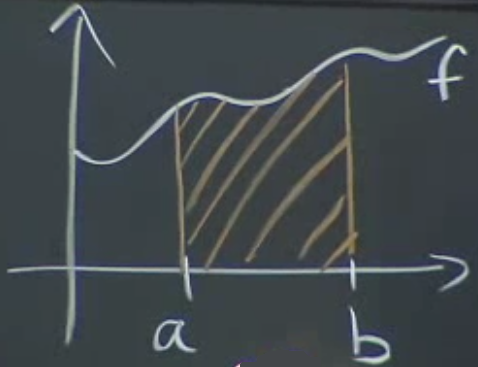
\includegraphics[height=2cm]{16_1.png}

Eger $f$ negatif ise o zaman alan eksen altinda yer alacaktir. 

Iki degiskenli fonksiyonlar icin benzer bir sey yapilabilir, 3 boyutlu
uzayda $z=f(x,y)$ fonksiyonumuzu grafikledigimizi dusunelim, bu bir yuzey olusturur,
yuzeyin altinda kalan ``hacim'' hesaplanabilir, ki bu hesap cift
entegraller ile mumkun olmaktadir. 

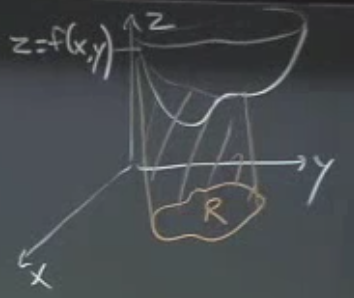
\includegraphics[height=3cm]{16_2.png}

Cift entegral icin $f(x,y)$'miza bakiyoruz, sonra ``uzerinden entegrasyon
isleminin yapilacagi'' bolge $R$'i seciyoruz. Tek entegraldeki $[a,b]$
araligi gibi, ama bu sefer bolge bir cizgi degil, bir alan. Entegral soyle
gosteriliyor 

\[ \int \int_R f(x,y) dA \]

Formulde $dA$'nin anlami ``$A$ alaninin bir parcasi'' demek. Hesaplama
vakti gelince bu notasyonun daha somut halini gorecegiz. 

Biraz daha matematiksel / teorik / detayli (rigorous) olarak bakmak
gerekirse; tek entegralde $[a,b]$ araligini ufak parcalara bolup, o
bolumlerin genisligini $f$ ile carptigimizi ve sonuclari birbirine
topladigimizi hayal ediyorduk. 

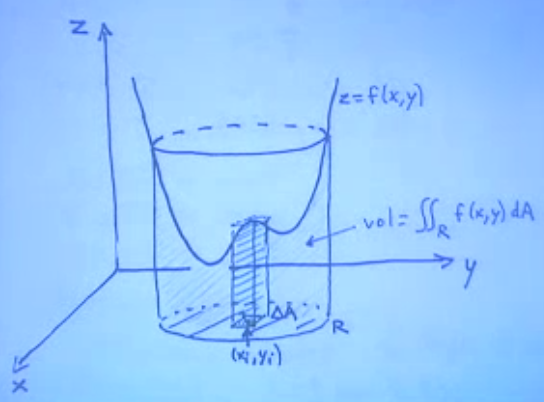
\includegraphics[height=4cm]{16_3.png}

Cift entegralde bu ufak bir kenari $\Delta x$ diger kenari $\Delta y$ olan
bir dikdortgen alani, $\Delta A$. Sonra $\Delta A$'yi o noktadaki $f$ ile
cariyoruz, ve resimde cizgili gosterilen hacmi buluyoruz. Tum entegral icin
bu hacimleri topluyoruz. Entegral matematiksel olarak bir limit olarak
gosteriliyor, yani $\Delta A$ gitgide ufaliyor. 

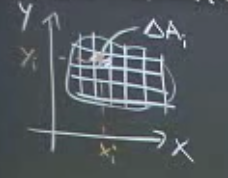
\includegraphics[height=3cm]{16_4.png}

Toplam soyle gosterilebilir

\[ \sum_i f(x_i,y_i) \ \Delta A_i \]

ve $\Delta A \to 0$ uzerinden limit aliyoruz, cift entegrali elde ediyoruz. 

Tabii ki entegral hesabini yaparken, tek ya da cift olsun, her seferinde
ufak parcalara bolup, toplam ile ugrasmiyoruz. Entegral kavraminin bize
sagladigi formulsel kolayliklari kullaniyoruz.

Cift entegral formullerini kullanmak icin ``tarayici bir duzlem'' hayal
edebiliriz. Mesela alttaki resimde $yz$ duzlemine paralel duzlemin arkadan
one dogru onune gecerek her seyi taradigini dusunelim, her duzlem $x=x_0$'a
tekabul ediyor, o zaman tarama sirasinda farkli $x_0$'lar kullaniyoruz. 

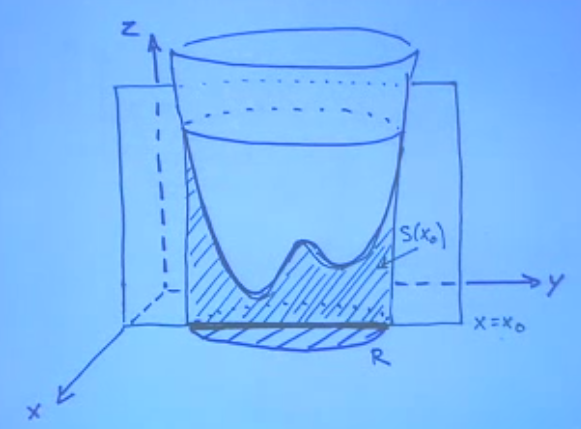
\includegraphics[height=4cm]{16_5.png}

Tek bir $x_0$ ``fotografina'' bakarsak, o duzlemin uzerinde dusen $f$
yansimasinin altindaki alanin normal (tek) bir entegral olarak
hesaplanabilecegini gorebiliriz. One dogru her hareket bir $\Delta x$ ise,
oradan her ufak hareketin hacmini buluruz. Tum bu ufak hacimleri toplarsak,
toplam hacmi elde ederiz. Fotograftaki her alana $S(x)$ adi verelim.

Yani 

\[ Hacim = \int S(x) dx \]

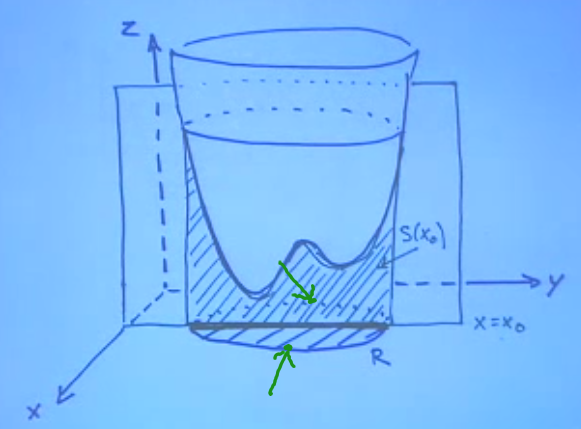
\includegraphics[height=3cm]{16_6.png}

Taramanin sinirlari ise ustteki yesil oklarla gosteriliyor. 












\end{document}
